\section{Introduction to SAR}

Synthetic aperture radar (SAR) is a method of radar imaging that allows for a greater dimension of radar aperture than is possible in a single element or an array of elements. This is generally achieved by mounting a radar transceiver to a moving platform and moving it past the target to be imaged however the transceiver can be stationary and the target moved past it. The image uses the relative movement between the platform and the target to build up an image based on the responses received and then time multiplexing all the responses. This movement, and hence the larger aperture created, allows for a finer spatial resolution than can be achieved by more conventional beam scanning radar. These images can be useful for a variety of applications such as remote mapping of the surface of the Earth for glaciology and geology among others. Interferometric SAR can also be used to create elevation maps by taking two measurements from different positions and comparing the differences.
Simulating a SAR image is desirable as flight time can be expensive and time consuming to get quality images so defining the flight paths and angles before any imaging is carried out saves both time and money. \par
There are two main methods of imaging using SAR. These are stripmap and spotlight imaging. Stripmap imaging SAR keeps the radar beam fixed at 90\degree to the direction of travel of the platform to which it is mounted, giving an even resolution image over the entire imaging area. Spotlight SAR uses beam steering in order to focus on one specific area to increase image resolution in that area, at the expense of image resolution in other areas. This extra time spent focusing on the single area increases the synthetic aperture length for that section only which increases the resolution.

\begin{figure}
	\centering
	\begin{subfigure}{.5\textwidth}
	\centering
	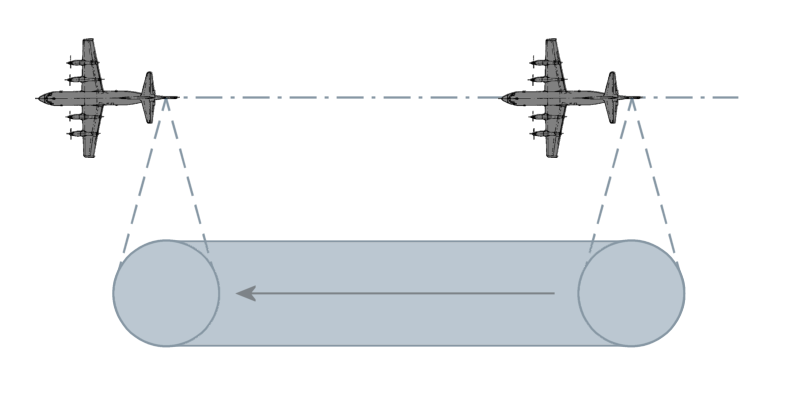
\includegraphics[width=0.45\linewidth]{../figures/sar_stripmap}	
	\caption{SAR in stripmap operation}
	\label{subfig:sar_stripmap}
	\end{subfigure}%
	\begin{subfigure}{.5\textwidth}
	\centering
	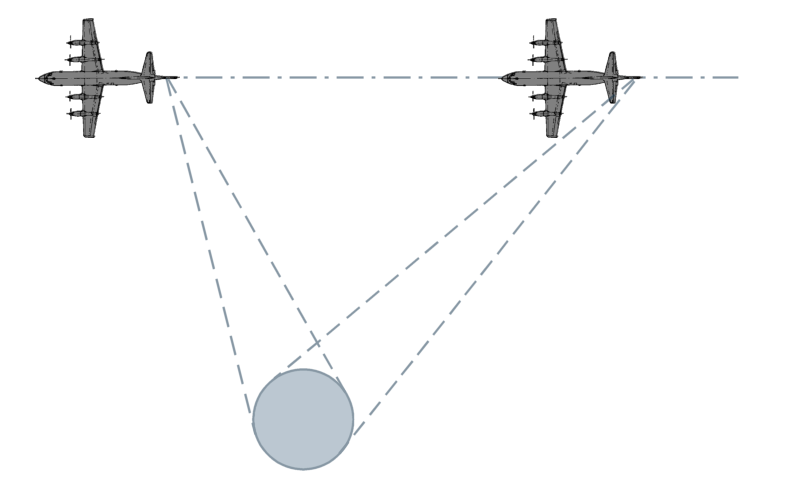
\includegraphics[width=0.45\linewidth]{../figures/sar_spotlight}	
	\caption{SAR in spotlight operation}
	\label{subfig:sar_spotlight}
	\end{subfigure}
	\caption{The two main modes of operation of SAR, reproduced from \cite{wolffSyntheticApertureRadar2012}}
	\label{fig:sar_modes}

\end{figure}

\subsubsection{The SAR radar equation}
There are two main approaches to SAR, focused and unfocused SAR. These differ in how they consider shifts in the response phase, as focused SAR only takes into account the Doppler shift across the aperture, while focused SAR takes into account the phase shift in the beam due to the change in range caused by the target passing through the beam. This means that the resolution of the image is determined by the length of the entire synthetic aperture, as opposed to in unfocused SAR where the resolution is a function of the shortest range between the platform and the target as well as the wavelength of the signal. The resolution of focused SAR is wavelength independent. The derivation of this can be found in Appendix \ref{appen:derivations}. Also in this appendix is a derivation of the radar equation both generally and then to the more specific version for SAR. The more general form of the radar equation for a single pulse is given as \[ \text{SNR} = \frac{P_t G^2 \lambda ^ 2 \sigma _b}{(4\pi)^3R^4kT_{sys} B} = \frac{P_t A_e^2 \sigma_b}{4\pi\lambda^2kT_{sys}BR^4}\] which gives the signal-to-noise ratio for a single pulse, where \gls{Pt} is the transmitted power, \gls{G} is the gain of the system, \gls{Ae} is the effective aperture area, \gls{lambda} is the wavelength of the signal, \gls{sigmab} is the radar cross-section, \gls{R} is the signal range, \gls{k} is Boltzmann's constant, \gls{Tsys} is the system noise temperature and \gls{B} is the bandwidth of the system. This can then be adapted to the SAR-specific radar equation by increasing the number of pulses \gls{n} to give \[\text{SNR} = \frac{P_t A_e^2 \sigma_b n}{4\pi \lambda^2kT_{sys}BR^4}\] and hence the signal-to-noise ratio of a distributed target is given by \[\text{SNR}=\frac{P_{av} A_e^2 \sigma^0\Delta R_g \Delta x t_{obs}}{4\pi\lambda^2kT_{sys}R^4} \text{     or     } \text{SNR} = \frac{P_{av}A_e^2\sigma^0\Delta x\lambda^3}{(4\pi)^3R^3kT_{sys}2v_p} \] where \gls{Pav} is the average power across all pulses, \gls{DeltaRg} is the ground range resolution of the system, \gls{tobs} is the observation time of the target and \gls{vp} is the platform velocity. The sensitivity of a SAR system can be expressed as the noise equivalent \gls{sigma0}, which is the value of \gls{sigma0} at the maximum range to give a signal-to-noise ratio of 1 (or 0 dB) \cite{watsonEE40136RadarSystems2020}.

\begin{figure}
\centering
\begin{subfigure}{.5\textwidth}
\centering
	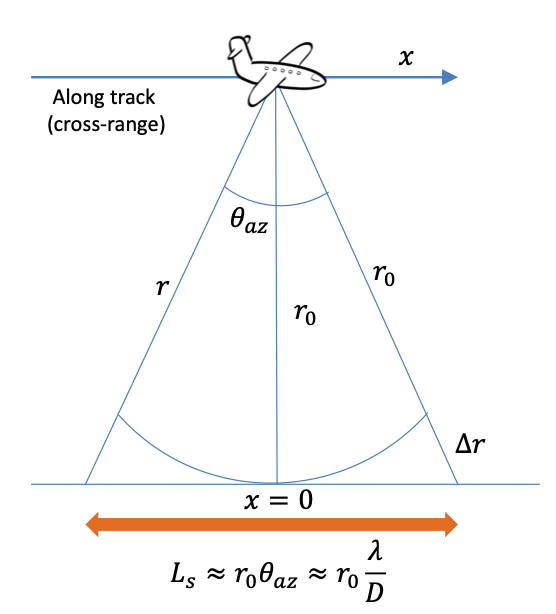
\includegraphics[width=0.9\linewidth]{../figures/sar_along_track_res}
\caption{Along-track/Cross-range SAR Resolution, reproduced from \cite{watsonEE40136RadarSystems2020}}
\label{subfig:sar_along_track}

\end{subfigure}%
\begin{subfigure}{.5\textwidth}
	\centering
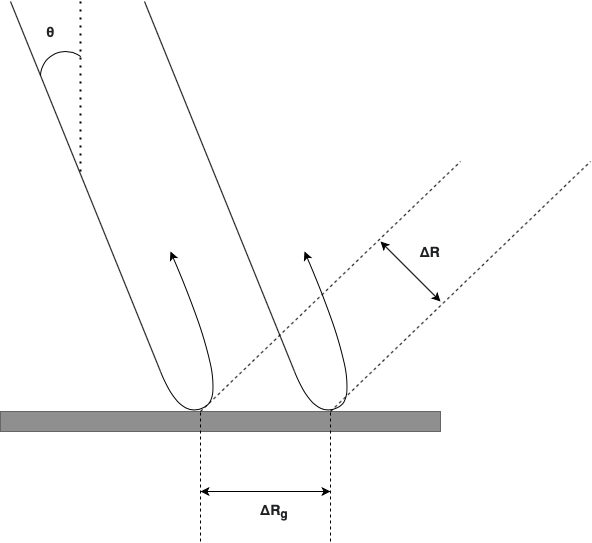
\includegraphics[width=0.9\linewidth]{../figures/down_range}	
\caption{Down-range SAR resolution, adapted from \cite{richardsRemoteSensingImaging2009}}
\label{subfig:down_range_SAR}
\end{subfigure}
\caption{Cross-sections of both dimensions of SAR range}
\label{fig:sar_range_cross_section}
\end{figure}


\subsubsection{SAR Image Artefacts}
There are a few artefacts that can arise as part of SAR imagery (and radar imagery in general). Some of these, such as range ambiguities, aren't relevant in this case due to the fact that all the targets being imaged are static and this is only a real issue in moving objects. Some artefacts will need to be considered though. The first of these is speckle, which is a result of the fact that the energy arriving at the pixel is pretty coherent, so it has a single phase on arrival at said pixel. Generally the pixel will be the sum of multiple scatterers as opposed to one single scatterer, meaning that it is likely to be affected by background reflections and so result in a relatively noisy image. This can be fixed in real world applications by splitting the SAR antenna into multiple sections and take the same image with each section. This then allows for the pixel values to be averaged out, hopefully removing the speckle at the cost of some resolution \cite{richardsRemoteSensingImaging2009}. \par 
Another image artefact that will need to be considered can be caused by strong scatterers that means that the signal is reflected multiple times before returning to the receiver. This can be seen most strongly with a bridge over water as it involves both a hard target in the bridge and a dihedral reflection from the water. This mostly occurs when the target is aligned with the path of the platform and the multiple reflections can cause the bridge to appear multiple times in the image due to the multiple bounces taken by the signal increase the Doppler shift presented when it is filtered on reception. The same signal is in essence received multiple times and so the algorithm reads it as different displacements for the same target \cite{richardsRemoteSensingImaging2009}. \par
Finally, some distortions can be created due to the geometry of the radar beam. Targets nearer the platform can appear compressed on the output image as the ground range in that location is greater but in the final image is represented in the same amount of image space as targets further away. Similarly, given a tower, reflections from the top of the tower will return to the platform before reflections from the bottom, causing the tower to appear to lean over towards the radar \cite{richardsRemoteSensingImaging2009}.
